\chapter{Transfer Learning}

\section{Transfer learning}
Transfer learning is a powerful technique to obtain results quickly when using deep CNNs. Here we will only take a look at transfer learning within the domain of deep CNNs, but it is a technique that has been successfully applied to many other domains of machine learning as well.

To give a formal definition of transfer learning, we will follow the definitions provided in \citep{transferSurvey2010}. Let $\mathcal{D}$ be a domain, which consists of a feature space $\mathcal{X}$ and a marginal probability distribution P($\mathcal{X}$). For a given domain, a task $\mathcal{T}$ = {$\mathcal{Y}$, f$\mathcal(X)$} consist of a label space $\mathcal{Y}$ for the inputs and of a predictive function $f(x)$ which produces predictions for all pairs ${x_i, y_i}$ where $x_i \in \mathcal{X}$ and $y_i \in \mathcal{Y}$. Given a source domain $\mathcal{D}_S$, a source task $\mathcal{T}_S$, a target domain $\mathcal{D}_T$ and a target task $\mathcal{T}_T$, where target and source are disjoint, transfer learning tries to improve the performance of $f_T(x)$ using $\mathcal{D}_S$ and $\mathcal{T}_S$.

The idea behind transfer learning is to train on a related task to the end task first. Then the network weights in the model for the actual task are initialized to those of the model we are transferring from, so the training of the original model is a pre-step to the real task. Since training the models on ImageNet \citep{imagenet} scale datasets is not generally feasible due to their large number of parameters and long training time, one of the pre-trained models is picked and then fine-tuned. Fine-tuning a classifier means taking the examples for the final task, and training the network on those, updating the original classifier at the same time. The transfer learning approach differs significantly from the traditional learning model, where each task requires a separate model that learns from the given data using random weights. Since image inputs are often very high dimensional, the traditional approach may not work in many cases. The pre-training allows for focusing on data that provides answers to the actual task and not on learning low-level features, which the ImageNet classifiers would already have learned.

\begin{figure}[h!] 
\centering 
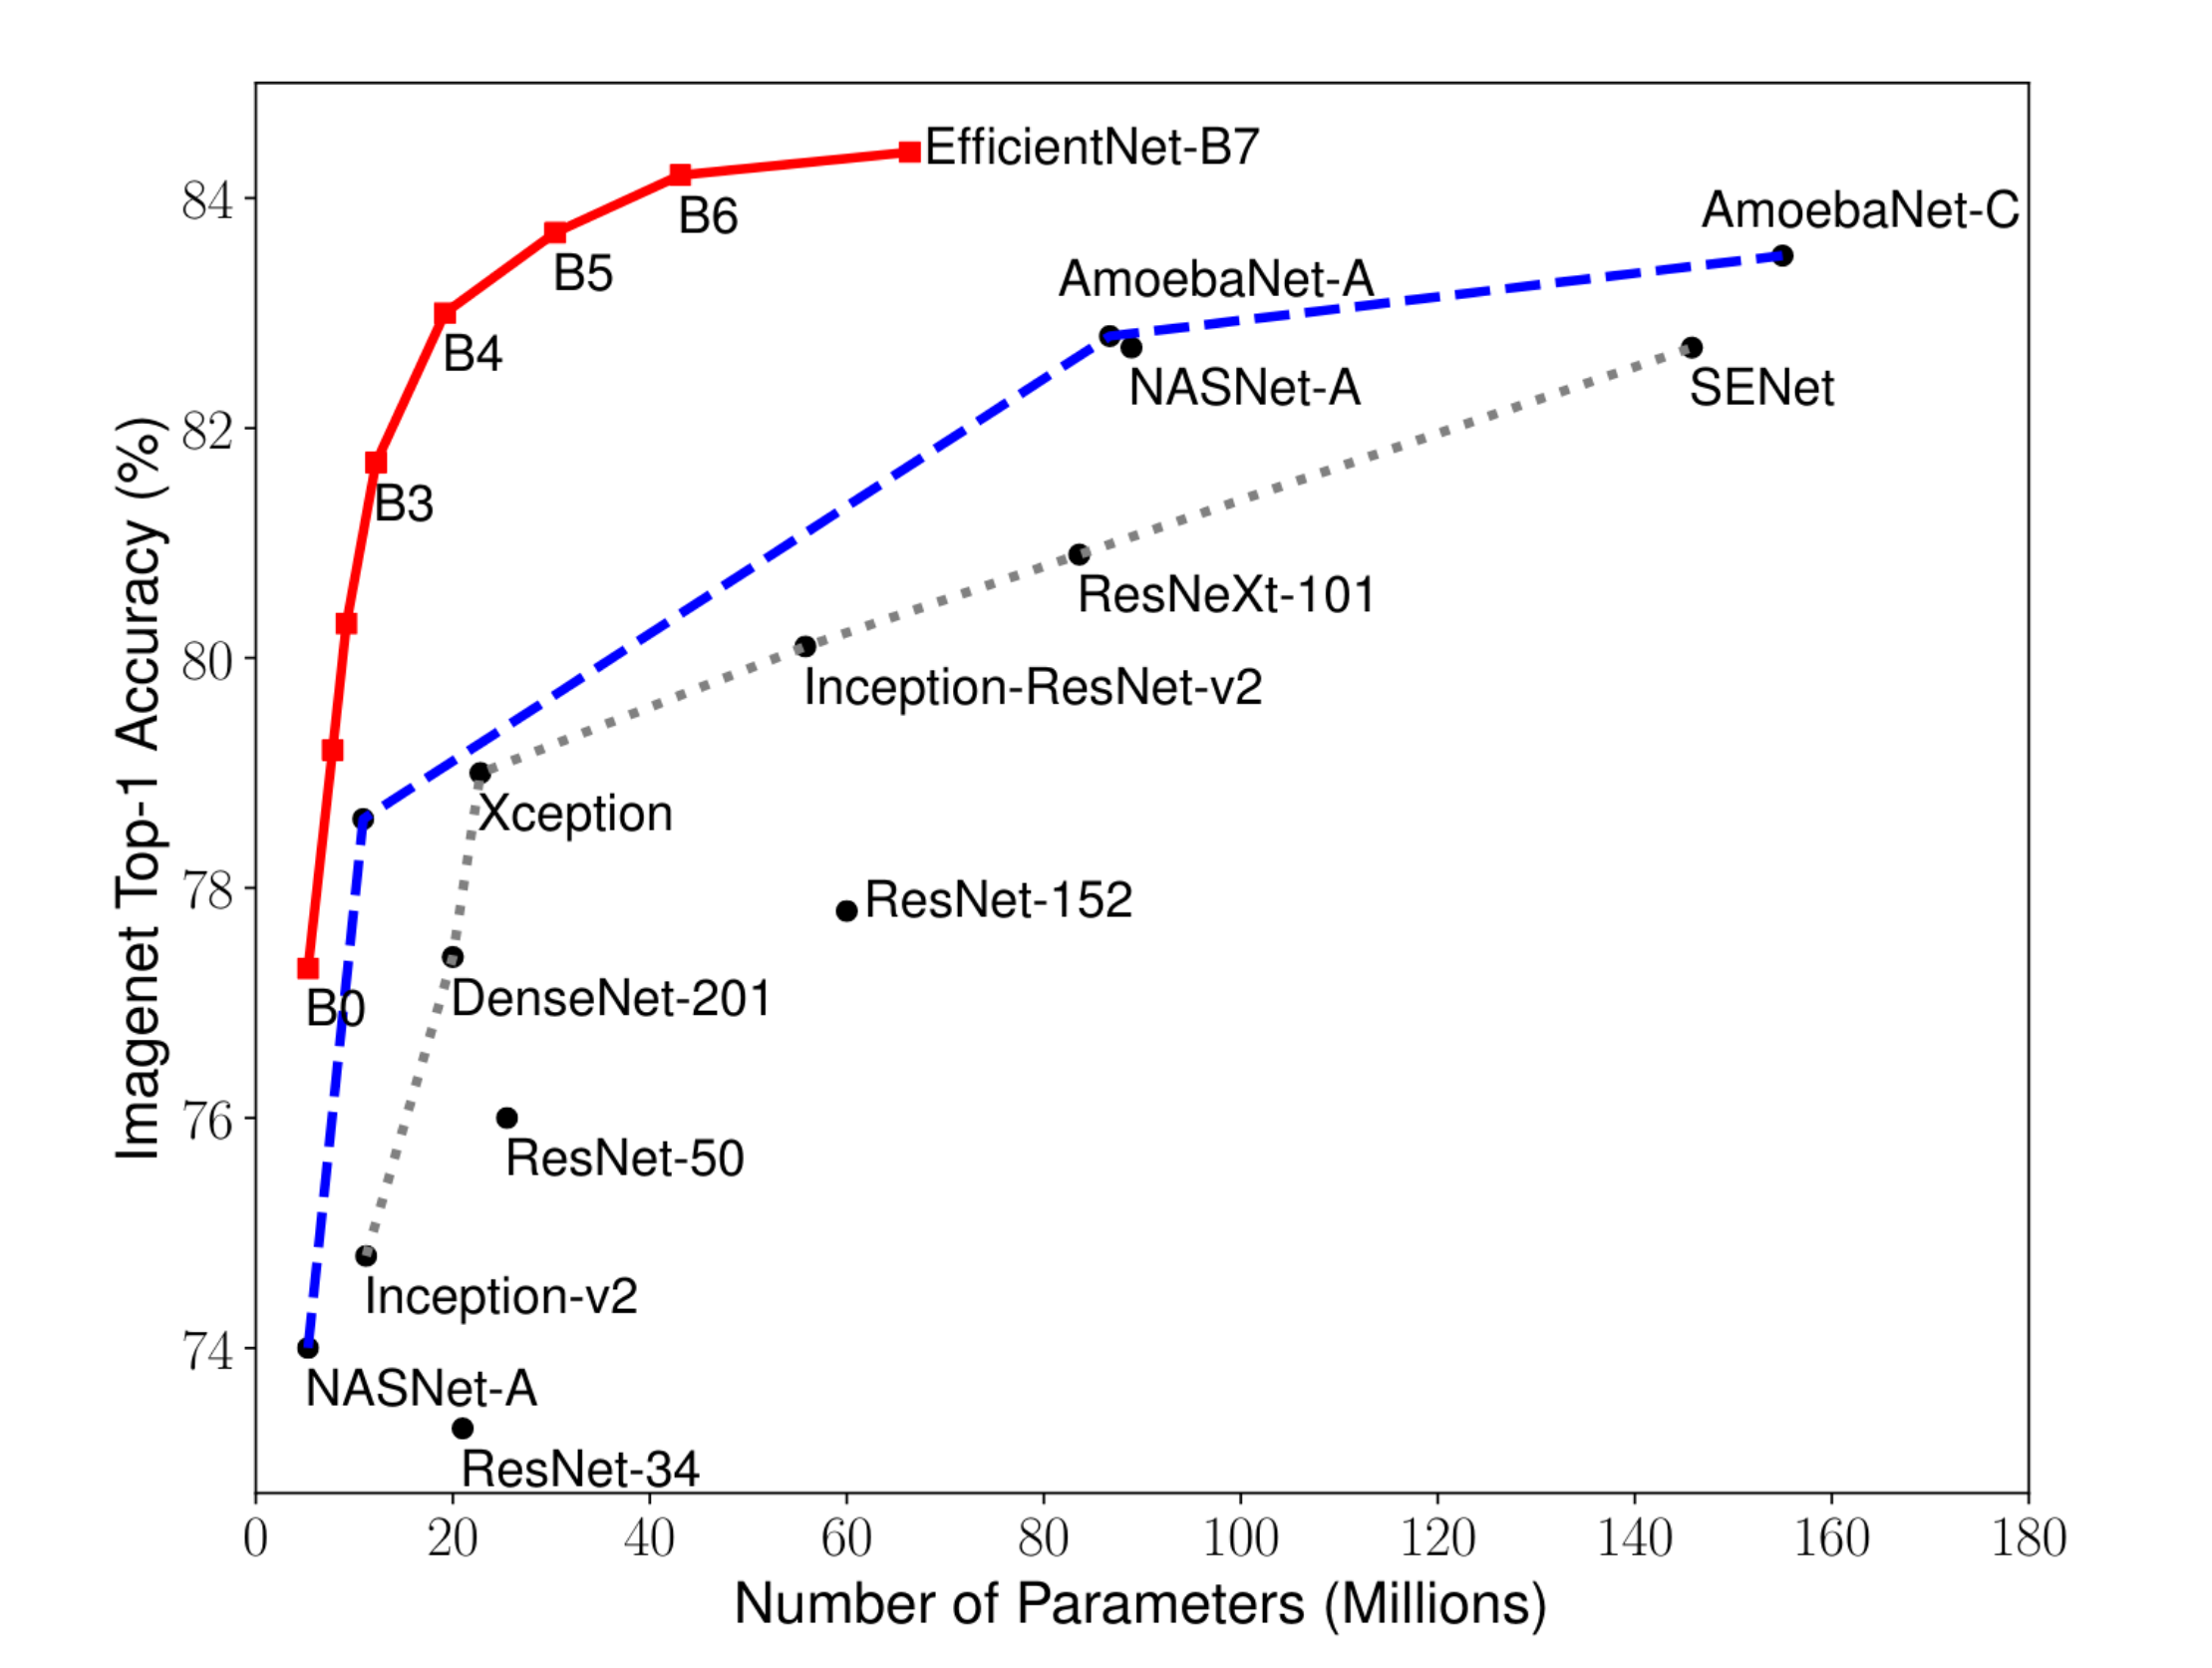
\includegraphics[width=0.8\textwidth]{imgs/imagenet_parameters.png}
\caption{Number of parameters in popular ImageNet classifiers. Figure from \citep{efficientNet}.\label{fig:params}}
\end{figure}

Picking which classifier to use as a base is often problem-dependent. As it is not possible to declare one network structure to be the best at all tasks, picking the best model to start with usually requires the user to compare different architectures and weighing the requirements for the problem at hand. Often though, the larger models will perform better, and there exists a correlation between performing well on ImageNet and being a good transfer learning model \citep{betterTransfer}. Though as can be seen in figure 2.1, better performance often comes at the cost of many more parameters, requiring more memory to train the model. Though just the number of parameters is not the only thing to compare as the throughput of a Resnet50 \citep{resNet} turns out to be about three times as large as the throughput of an EfficientNet-B4 \citep{efficientNet} even though they have a similar amount of parameters \citep{classifierPerformance}. So in the case of time-constrained inference environments, also the time required for an inference has to be taken into account when picking models.

If there is enough data, it turns out that using a pre-trained network does not provide any benefits in terms of the converged model accuracy, but it is not detrimental to performance either \citep{rethinkTransfer}. When training sufficiently long on a sufficient amount of data, the pre-trained and randomly initialized networks converged to similar accuracies but required significantly different amounts of training resources. Still, this does not mean that pre-training is useless by any means as the saved resources and getting models to converge faster are essential factors for progress, and of course, in many cases, training from scratch will not provide satisfying results.

